% N.B. : Assurez-vous de compiler ce fichier en employant "pdflatex" afin que les images soient incluses.

% Tout commentaire est bienvenu et devrait être adressé à "support@dms.umontreal.ca".

\documentclass[12pt,travaildirige,nobabel, twoside]{dms} 
% La commande précédente charge la classe "dms.cls" avec les options suivantes : police de caractères en 12 pts, écriture française, format adapté à une thèse de doctorat et impression recto-verso.

% Voici la liste exhaustive des options disponibles :

% maitrise			mémoire de maîtrise;
% phd				thèse de doctorat;
% rapport			rapport de stage;
% travaildirige		travail dirigé;
% nobabel			écriture en anglais seulement;
% oneside			impression recto;
% twoside			impression recto-verso.
\usepackage[english]{babel}
\usepackage{adjustbox}    
\usepackage[utf8]{inputenc}		% Indique à LaTeX que l'encodage du fichier source (.tex) est UTF-8. 
\usepackage[T1]{fontenc}		% Assure un enregistrement adéquat des accents dans le fichier compilé (.pdf).
\usepackage{lmodern}			% Charge la fonte vectorielle "Latin Modern", une version de la fonte par défaut "Computer Modern", qui supporte les caractères latins.
\usepackage{graphicx,amsmath,amsfonts,amssymb,setspace,subfigure,color}
% graphicx		Pour importer des images (PDF, JPG, PNG).
% amsmath		Écriture selon les normes de l'AMS.
% amsfonts		Fontes additionnelles de l'AMS.
% amssymb		Écriture des symbols de l'AMS.
% setspace		Permet de régler la distance interligne dans le document.
% subfigure		Simplifie l'inclusion de figures côtes-à-côtes.
% color			Pour l'utilisation de couleurs dans le texte.

\definecolor{mygreen}{RGB}{28,172,0} % color values Red, Green, Blue
\definecolor{mylilas}{RGB}{170,55,241}

\usepackage[pdfpagemode=UseNone,pdfstartview={XYZ null null null}]{hyperref}			% Cette extension permet l'insertion d'hyperliens dans votre document pdf.
 \definecolor{dark-red}{rgb}{0.4,0.15,0.15}												% Ici, trois couleurs sont définies et seront utilisées pour colorer les "hyperliens".
 \definecolor{dark-blue}{rgb}{0.15,0.15,0.4}
 \definecolor{medium-blue}{rgb}{0,0,0.5}
 \hypersetup{colorlinks,linkcolor={dark-red},citecolor={dark-blue},urlcolor={medium-blue}}

\usepackage[longnamesfirst,numbers,square]{natbib}		% Pour l'utilisation de bibliographies BibTeX au format "auteur-année".

% Numérotation des équations par section et numérotation des tableaux et figures par chapitre.
\usepackage{listings}

\numberwithin{equation}{section}
\numberwithin{table}{chapter}
\numberwithin{figure}{chapter}

% Définition des environnements utiles pour un mémoire scientifique.

\newtheorem{corollary}{Corollaire}[section]
\newtheorem{mydef}{Definition}[section]
\newtheorem{example}{Exemple}[section]
\newtheorem{lemma}{Lemme}[section]
\newtheorem{proposition}{Proposition}[section]
\newtheorem{remark}{Remarque}[section]
\newtheorem{theorem}{Theorem}[section]

% Si vous préférez que les corollaires, definitions, théorèmes, etc. soient numérotés par le même compteur, utilisez plutôt ce bloc de commandes : 

%\newtheorem{corollary}{Corollaire}[section]
%\newtheorem{definition}[corollary]{Définition}
%\newtheorem{example}[corollary]{Exemple}
%\newtheorem{lemma}[corollary]{Lemme}
%\newtheorem{proposition}[corollary]{Proposition}
%\newtheorem{remark}[corollary]{Remarque}
%\newtheorem{theorem}[corollary]{Théorème}

\onehalfspacing				% Fixe la distance interligne à "1.5". Pour une interligne double, utilisez plutôt "\doublespacing".

\allowdisplaybreaks			% Cette commande autorise LaTeX à briser les blocs d'équations, permettant ainsi une couverture plus uniforme des pages.


%
% ---------  D É B U T  D U  D O C U M E N T  ---------
%


\begin{document}

% La commande "\brouillon" imprime, au bas de chaque page, la date ainsi que l'heure de la dernière compilation de votre fichier.

%\brouillon            

% Voici les variables pour la création de votre page titre.

\title{Risk Measure for the Generalized Normal Laplace Distributions }
\author{Dora Fugère}
\copyrightyear{2015}
\date{\today}									% Date de dépôt du document.
\president{Nom du président du jury}
\directeur{Nom du directeur de recherche}
%\codirecteur{Nom du codirecteur}     			% Optionnel.
\membrejury{Nom du membre du jury} 
\examinateur{Nom de l'examinateur externe}		% Obligatoire pour la thèse.
%\membresjury{alpha, beta, gamma}				% Optionnel.
%\plusmembresjury{psi, zeta, omega} 			% Optionnel.
\repdoyen{Nom du représentant du doyen} 		% Obligatoire pour la thèse.
\dateacceptation{Date d'acceptation}
\sujet{finance mathématique et computationnelle}							% Votre discipline de recherche, soit "mathématiques" ou "statistique".
%\orientation{mathématiques fondamentales}		% Cette commande est optionnelle. Les choix courants sont : "mathématiques fondamentales", "mathématiques de l'ingénieur" et "mathématiques appliquées".

% Fin des variables à définir. La commande "\maketitle" créera votre page titre.

\pagenumbering{roman}
\maketitle    
 


\chapter*{Sommaire} 	% La commande "\chapter*" crée un chapitre sans numéro, contrairement à la commande "\chapter" régulière.

Le but de ce projet dirigé est d'étudier l'espérance conditionnelle unilatérale (Tail-Value-at-Risk) de la distribution normale généralisée de Laplace (GNL).
Nous proposons une méthode numérique pour calculer l'espérance conditionnelle unilatérale basée sur l'approximation numérique de la fonction de densité et  sur l'approximation numérique de la fonction de répartition.
L'estimateur numérique obtenu pour l'espérance conditionnelle unilatérale nous donne des valeurs qui sont toujours dans un intervalle de confiance créé par une méthode de type bootstrap.
Les résultats de la simulation ainsi que la plupart des programmes sont présentés.\\

\bigskip
 
\noindent Mots clés: Valeur à risque, espérance conditionnelle unilatérale, distribution normal généralisée de Laplace, distribution de Laplace, approximation numérique.	% N.B. : La commande "\noindent" force LaTeX à ne pas indenter le nouveau paragraphe.



\chapter*{Summary}

The purpose of this directed project is to study the Tail-Value-at-Risk (TVaR) of the generalized normal Laplace distribution (GNL).
We propose a numerical method to evaluate the TVaR based on the numerical approximation of the probability density function and on the numerical approximation of the cumulative density function.
The numerical estimator obtained for the TVaR gives us values that are always inside the confidence interval created using a bootstrap method.
Simulation results and the programmes are provided. \\

\bigskip
\noindent Keywords: Value-at-Risk, Tail-Value-at-Risk, Conditional Tail Expectation, generalized normal Laplace distribution, numerical approximation.

\tableofcontents				% Table des matières.
\listoffigures					% Liste des figures.
\listoftables					% Liste des tableaux.



\chapter*{Acknowledgements}
I would first like to thank my supervisor Dr. Louis G. Doray for his guidance, his patience, his motivation, and knowledge. I would also like to thank my family for their support. 

% Fin des pages liminaires. À partir d'ici, les premières pages des chapitres ne doivent pas être numérotées.

\NoChapterPageNumber 
\pagenumbering{arabic}

% Voici maintenant le chapitre d'introduction.



\chapter*{Introduction}

%a reformuler.
%Reed (2006, 2007) introduced a new distribution, the generalized normal %Laplace (GNL) and showed its usefulness in modeling the size distributions %of various phenomena arising in areas such as economics, finance, %geography, physical sciences and geology. Properties such as infinite %divisibility, skewness and excess kurtosis make the GNL distribution a good %candidate model in option pricing.\\

Option pricing has been studied a lot. A candidate model for the interest rate process in option pricing was introduced by Reed (2006, 2007), the generalized normal Laplace (GNL) distribution. The GNL has some key properties that make it a good candidate model in option pricing; these properties are infinite divisibility, skewness, and excess kurtosis.\\


The closed form for the probability density function (pdf) of the generalized normal Laplace remains unknown. For this reason, we need to turn to numerical calculations whenever we want to study the GNL. Now if we use this distribution as an option pricing model, we want to be able to manage the risk that goes with such model.\\

The major aim of this research project is to examine the numerical methods available to evaluate the Tail-Value-at-Risk (sometime called \textit{Conditional Tail Expectation}). We explain how to obtain numerical approximations of the probability density function and the cumulative distribution function. We develop a method for evaluating the Value-at-Risk (VaR) of a generalized normal Laplace distribution based on the Newton-Raphson method. 




\chapter{Generalized normal Laplace distribution}




\section{The charactheristic function and the moment generating function}


We start by defining a key tool of probability theory, that is the characteristic function. \\

\begin{mydef}\leavevmode \\
\textbf{The characteristic function} of a random variable \textbf{X} is defined as \\
\begin{equation}
 \phi_\textbf{X}(t)=E[e^{it\textbf{X}}]=E[cos(t\textbf{X})+isin(t\textbf{X})] \end{equation} \\ with \begin{math} i=\sqrt{-1} \end{math} and E being the expected value . \\ 
\end{mydef}
\nocite{lossmodel}
We now define a similar function, that is the moment generating function.\\

\begin{mydef}
\textbf{The moment generating function} of a random variable \textbf{X} is defined as \\
\begin{equation}
M_\textbf{X} =E(e^{\textbf{X}t})   \text{      for all t$ \in\mathbb{R}.$}
\end{equation}
\end{mydef}
\subsection{Properties of the characteristic function and the moment generating function}

The first property is to guaranty the existence of the characteristic function for every random variables.
\begin{proposition}
Let \textbf{X} be a random variable. Then the characteristic function $\phi_\textbf{X}$ exist. 
\end{proposition}
\begin{proof}
We first notice that 
\begin{equation}
\phi_\textbf{X}=E[e^{it\textbf{X}}]=\int_{-inf}^{inf}e^{it\textbf{X}}dF_{\textbf{X}}(x)
\end{equation}
with the integral been the Riemann-Stieltjes integral.
We also notice that
\begin{equation}
|e^{it\textbf{X}}|=|cos(t\textbf{X})+isin(t\textbf{X})|=\sqrt{cos(t\textbf{X})^2+sin(t\textbf{X})^2}=1.
\end{equation}
Now since
\begin{equation}
|\phi_\textbf{X}|=|E(e^{\textbf{X}t})|\leq \int_{-inf}^{inf}|e^{it\textbf{X}}|dF_{\textbf{X}}(x)=\int_{-inf}^{inf}dF_{\textbf{X}}(x)=1
\end{equation}
we can conclude that $\phi_\textbf{X}$ always exist since the absolute value of the integral is bounded\nocite{distquadGNL}.
\end{proof}

One of the main use of the characteristic function is to study the sums of independent random variables and to identify the resulting distribution.\\

The following proposition and theorem are used to show the continuity and derivability of the characteristic function.

\begin{proposition}
Let \textbf{X} be a random variable with characteristic function $\phi_\textbf{X}$. Then $\phi_\textbf{X}$ is uniformly continuous on $\mathbb{R}$\nocite{proba}.
\end{proposition}

\begin{proof}
See Athreya and Lahiri\citep{proba}.
\end{proof}


\begin{theorem}
Let \textbf{X} be a random variable with characteristic function $\phi_\textbf{X}$. If $E[\textbf{X}]^r<\infty$ for some $r\in\mathbb{N}$, then $\phi_\textbf{X}$ is r-times continuously differentiable and 
\begin{equation}
\phi_\textbf{X}^{(r)}(r)=E(i\textbf{X})^r exp(it\textbf{X}), t\in\mathbb{R}\text{\nocite{proba}.}
\end{equation}
\end{theorem}

\begin{proof}
See Athreya and Lahiri\citep{proba}.
\end{proof}

The following theorem is a strong theorem of probability theory. This theorem is sometimes used in proving some version of the central limit theorem. \\

\begin{theorem}
Let \textbf{X} be a random variable such that $M_\textbf{X} (s)<\infty$ for some $|s|<s_0$, for some $s_0>0$. Then $E[\textbf{X}^n]<\infty$ for all n, and $M_\textbf{X} (s)$ is analytic for $|s|<s_0$ with
\begin{equation}
M_{\textbf{X}}(s)=\sum^\infty_{n=0}E[\textbf{X}^n]s^n/n!.
\end{equation}
In particular, the $r^{th}$ derivative at s=0 is given by $M_{\textbf{X}}^{r}(0)=E[\textbf{X}^r]$\nocite{rigprob}.
\end{theorem}

\begin{proof}
See Rosenthal\citep{rigprob}.
\end{proof}


The following proposition is useful when working with sum of independent random variable.\\

\begin{proposition} \label{prop:convo ind}
Let \textbf{X} and \textbf{Y} be two independent random variables.
Then 
\begin{equation}
\phi_{\textbf{X}+\textbf{Y}}(t)=\phi_\textbf{X}\cdot\phi_\textbf{Y}(t), t\in\mathbb{R}\text{\nocite{proba}.}
\end{equation}
\end{proposition}

\begin{proof}
See Athreya and Lahiri\citep{proba}.
\end{proof}

The next theorem is also a strong theorem of probability theory, it takes full use of  proposition \ref{prop:convo ind} and gives a tool for identifying the distribution of a sum of independent random variables.\\

\begin{theorem} \label{thm:charactheristic function}
Let \textbf{X} and \textbf{Y} be random variables with characteristic function $\phi_\textbf{X}$ and $\phi_\textbf{Y}$ respectively.
If $\phi_\textbf{X} =\phi_\textbf{Y}$, then \textbf{X} = \textbf{Y} and conversely (the equality holds in distribution and conversely)\nocite{distquadGNL}.
\end{theorem}

\begin{proof}
See Shiryayev \citep{shiryayev}.
\end{proof}
\section{Definition of the distribution}

The generalized normal Laplace distribution is introduced by the following definition. \\

\begin{mydef}\leavevmode \\
\textbf{X} follows a \textbf{generalized normal Laplace} (GNL) distribution if its charactheristic function equals \\
\begin{equation}\label{eq:cf} \phi_\textbf{X}(t)=E[e^{it\textbf{X}}]=\bigg[\frac{\alpha \beta \exp({\mu it-\sigma ^2 t^2/2})}{(\alpha-it)(\beta+it)}\bigg]^{\rho} \end{equation} 
\noindent
where the parameter $\mu\in\mathbb{R}$ is a location parameter, the parameter $\sigma^2\in\mathbb{R}^+$ is a scale parameter, the parameter $\alpha\in\mathbb{R}^+$ and $\beta\in\mathbb{R}^+$ are affecting, respectively, the left tail and the right tail, and the parameter $\rho\in\mathbb{R}^+$ is a shape parameter. We will be using the notation \begin{math}\textbf{X}\sim GNL( \mu,\sigma^2,\alpha, \beta,\rho)\end{math}\nocite{distquadGNL}. \\

\end{mydef}



\section{Properties of the GNL distribution}

\subsection{Representation as a convolution}

\begin{proposition}\label{eq:convolution}
Let $\textbf{X}\sim GNL(\mu,\sigma^2,\alpha,\beta,\rho)$; then \textbf{X} has the following representation

\begin{equation}
\textbf{X}\stackrel{dist}{=}\rho\mu + \sigma\sqrt{\rho}\textbf{Z}+\frac{1}{\alpha}\textbf{G}_1-\frac{1}{\beta}\textbf{G}_2 
\end{equation}\\ with \textbf{Z}, $\textbf{G}_1$ and $\textbf{G}_2$  independent random variables with $\textbf{Z}\sim N(0,1)$ and $\textbf{G}_1,\textbf{G}_2$ following a gamma distribution with shape parameter $\rho$ and scale parameter 1\nocite{distquadGNL}.
\end{proposition}

\begin{proof}

	The characteristic function $\phi_\textbf{X}(t)$ given by \eqref{eq:cf} can be written as 
	\begin{equation}\begin{split}
	\phi_\textbf{X}(t)=exp(\rho\mu i t-\rho\sigma^2 t^2/2)\bigg[\frac{\alpha}{\alpha-it}\bigg]^\rho \bigg[\frac{\beta}{\beta +it}\bigg]^\rho\\  =exp(\rho\mu it)exp(-\rho\sigma^2 t^2/2)(1-it/\alpha)^{-\rho}(1+it/\beta)^{-\rho}\end{split}\end{equation}
	
	Let $\textbf{Z},\textbf{G}_1$ and $\textbf{G}_2$ be independent random variable, where \textbf{Z} has a normal distribution with mean 0 and variance $\sigma^2\rho$ and where $\textbf{G}_1 $ and $\textbf{G}_2$ follow gamma distribution with shape parameter $\rho$ and scale parameter 1.
	
	We now evaluate the characteristic function of these random variables.
	\begin{equation}
	\begin{aligned}
	\phi_{\textbf{Z}}(t)&=E[exp(it\textbf{Z})]=exp(-\frac{1}{2}\sigma^2t^2)\\
	\phi_{\textbf{G}_1}(t)&=\phi_{\textbf{G}_2}(t)=E[exp(it\textbf{G}_2)]=(1-it)^{-\rho}	
	\end{aligned}
	\end{equation}

	We let $ \textbf{Y}{=}\rho\mu + \sigma\sqrt{\rho}\textbf{Z}+\frac{1}{\alpha}\textbf{G}_1-\frac{1}{\beta}\textbf{G}_2 $ and we evaluate $\phi_\textbf{Y}(t)$.
	

	\begin{equation}
	\begin{aligned}
		\phi_\textbf{Y}(t)&=E[exp(it\textbf{Y})]=E[exp(it(\rho\mu + \sigma\sqrt{\rho}\textbf{Z}+\frac{1}{\alpha}\textbf{G}_1-\frac{1}{\beta}\textbf{G}_2)]\\
		&=E[exp(it\rho\mu)exp(it\sigma\sqrt{\rho}\textbf{Z})exp(it\frac{1}{\alpha}\textbf{G}_1)exp(-it\frac{1}{\beta}\textbf{G}_2)\\
		&=E[exp(it\rho\mu)]E[exp(it\sigma\sqrt{\rho}\textbf{Z})]E[exp(it\frac{1}{\alpha}\textbf{G}_1]E[exp(-it\frac{1}{\beta}\textbf{G}_2]\\
		&=exp(\rho\mu it)\phi_{\sigma\sqrt{\rho}\textbf{Z}}(t)\phi_{\frac{1}{\alpha}\textbf{G}_1}(t)\phi_{-\frac{1}{\beta}\textbf{G}_2}(t)\\
		&=exp(\rho\mu it)exp(-\rho\sigma^2 t^2/2)(1-it/\alpha)^{-\rho}(1+it/\beta)^{-\rho}
		\end{aligned}
	\end{equation}
We then have from theorem \ref{thm:charactheristic function} that \textbf{X} and \textbf{Y} follow the same distribution since they have the same characteristic function.


	\end{proof}
\subsection{Infinite Divisibility}

The infinite divisibility of a distribution is a powerful property.  If one can show that the GNL is infinitely divisible, then the sum of \textit{n} independent and identically distributed GNL will have a GNL distribution (with a change of parameter).\\

\begin{mydef}
A random variable \textbf{X} has an \textbf{infinitely divisible distribution} if and only if, for each n, there exist independent, identically distributed random variables $\textbf{X}_{n,k}$, $1 \le k \le n$, such that $\textbf{X}= \sum^n_{k=1}\textbf{X}_{n,k}$ for all n, or, equivalently, if and only if $\phi_\textbf{X}(t)=(\phi_{x_{n,1}}(t))^n$ for all n\nocite{distquadGNL}.\\
\end{mydef}

\begin{proposition}
The generalized normal Laplace distribution is infinitely divisible.
\end{proposition}

\begin{proof}
Let \begin{math}\textbf{X}\sim GNL( \mu,\sigma^2,\alpha, \beta,\rho)\end{math} and let \begin{math}\textbf{Y}= \sum^n_{k=1}\textbf{X}_{n,k}\end{math}, with \begin{math}=\textbf{X}_{n,k}\sim GNL( \mu,\sigma^2,\alpha, \beta,\frac{\rho}{n})\end{math} for $k=1\dots n$\\

We have \begin{equation}
\begin{aligned}
\phi_\textbf{Y}(t)&=\phi_{\sum^n_{k=1}\textbf{X}_{n,k}}(t)\\
&=E[e^{\sum^n_{k=1}\textbf{X}_{n,k}it}]=E[\Pi^n_{k=1}e^{\textbf{X}_{n,k}it}]\\
&=\Pi^n_{k=1}E[e^{\textbf{X}_{n,k}it}]\\
&=\Pi^n_{k=1}[\frac{\alpha \beta \exp{\mu it-\sigma ^2 t^2/2}}{(\alpha-it)(\beta+it)}]^{\frac{\rho}{n}}\\
&=[\frac{\alpha \beta \exp{\mu it-\sigma ^2 t^2/2}}{(\alpha-it)(\beta+it)}]^{\rho}=\phi_\textbf{X}(t)\\
\end{aligned}
\end{equation}

We then have from theorem \ref{thm:charactheristic function} that \textbf{X} and \textbf{Y} follow the same distribution since they have the same characteristic function, therefore \textbf{X} is infinitely divisible.
\end{proof}

\subsection{Unimodality of the generalized normal Laplace}\label{unimodal}

\begin{mydef}
A distribution is \textbf{unimodal} if its probability density function possesses an unique mode.
\end{mydef}

The unimodality of the GNL is unknown for the moment. Since there is no proof of unimadolity, we will study the change of the pdf curve of the GNL when changing the value of the parameters. We note that the curves shown bellow are generated using numerical approximation explained  in this research.\\ 

\clearpage

\begin{figure}[h!]
\caption {The effect of varying $\mu$ on the probability density function of $X\sim GNL(\mu,\sigma^2=2,\alpha=1,\beta=2,\rho=2)$}\label{fig:mu}
  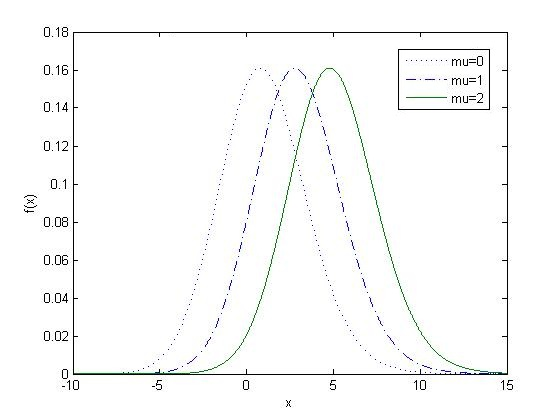
\includegraphics[width=10cm,height=10cm,keepaspectratio]{mu.jpg}
\end{figure}

Figure \ref{fig:mu} shows the effect of changing the value of $\mu$. Increasing the value of $\mu$ shifts the curve to the right, while decreasing the value of $\mu$ shifts the curve to the left.

\begin{figure}[h!]
\caption{The effect of varying $\sigma$ on the probability density function of $X\sim GNL(\mu=1,\sigma^2,\alpha=1,\beta=2,\rho=2)$}\label{fig:sigma}
  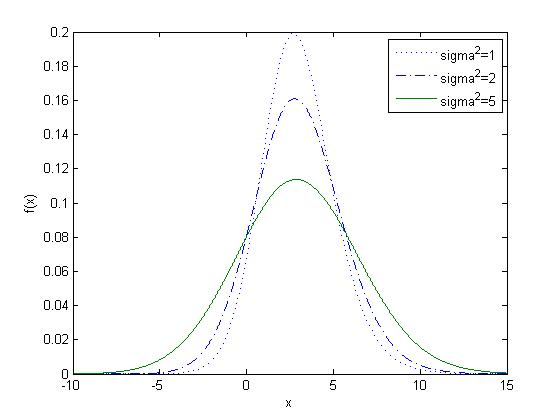
\includegraphics[width=10cm,height=10cm,keepaspectratio]{sigma.jpg}
\end{figure}

Figure \ref{fig:sigma} shows the effect of changing the value of $\sigma^2$. Increasing the value of $\sigma^2$ will result in a wider curve.\\ 
\clearpage
\begin{figure}[h!]
\caption {The effect of varying $\alpha$ on the probability density function of $X\sim GNL(\mu=1,\sigma^2=2,\alpha,\beta=2,\rho=2)$}\label{fig:alpha}
  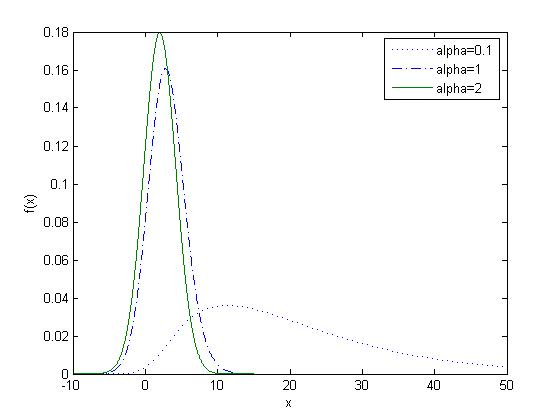
\includegraphics[width=10cm,height=10cm,keepaspectratio]{alpha.jpg}
\end{figure}

Figure \ref{fig:alpha} shows the effect of changing the value of $\alpha$. When $\alpha$ is small the upper tail is heavier. Having a big value of $\alpha$ will make the upper tail look like a normal distribution. As one might have expected given proposition \ref{eq:convolution}.\\


\begin{figure}[h!]
\caption {The effect of varying $\beta$ on the probability density function of $X\sim GNL(\mu=1,\sigma^2=2,\alpha=1,\beta,\rho=2)$}\label{fig:beta}
  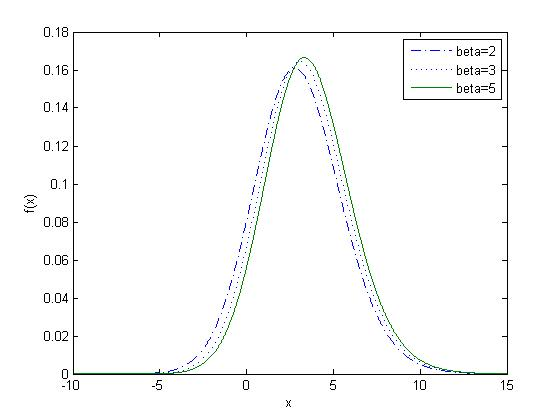
\includegraphics[width=10cm,height=10cm,keepaspectratio]{beta.jpg}
\end{figure}

Figure \ref{fig:beta} shows the effect of changing the value of $\beta$. The change in the value of $\beta$ affects the lower tail of the curve in the same way that the parameter $\alpha$ affects the upper tail of the curve. We note that bigger value of $\beta$ as less impact as can show figure \ref{fig:beta} whose value of $\beta$ are 2,3 and 5.\\

\begin{figure}[h!]
\caption {The effect of varying $\rho$ on the probability density function of  $X\sim GNL(\mu=1,\sigma^2=2,\alpha=1,\beta=2,\rho)$}\label{fig:rho}
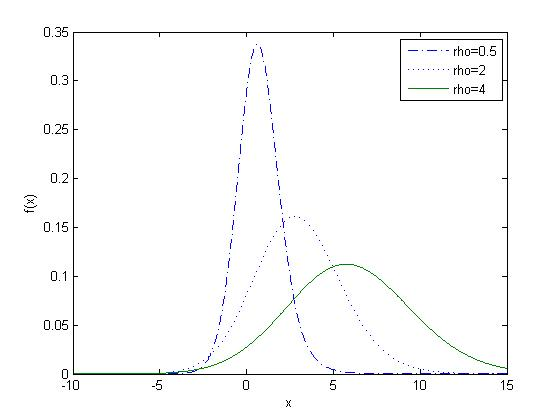
\includegraphics[width=10cm,height=10cm,keepaspectratio]{rho.jpg}
\end{figure}

Figure \ref{fig:rho} shows the effect of changing the value of $\rho$. Increasing the value of $\rho$ will have the same effect as increasing the value of $\mu$ and $\sigma^2$, thus resulting in a wider curve.\\

With all these figures, we believe the GNL is unimodal. When working with numerical approximation of the GNL, we are going to take as an assumption the unimodality of the distribution. However we are going to create a flag in the code that uses the unimodality of the distribution to prevent error, if we find a non-unimodal exemple.  
\clearpage

\section{Numerical method to determine the pdf and the cdf of the GNL}

Since there is no closed form of the pdf of the GNL, we are going to use numerical approximations to evaluate the pdf. We are going to use two different methods and use Matlab to test them.

\subsection{Using the Representation as a Convolution}
We know from proposition \ref{eq:convolution} that if \begin{math}\textbf{X}\sim GNL( \mu,\sigma^2,\alpha, \beta,\rho)\end{math} then \\
\begin{equation} 
\textbf{X}\stackrel{dist}{=}\rho\mu + \sigma\sqrt{\rho}\textbf{Z}+\frac{1}{\alpha}\textbf{G}_1-\frac{1}{\beta}\textbf{G}_2, 
\end{equation}\\ with \textbf{Z}, $\textbf{G}_1$ and $\textbf{G}_2$  independent random variables with $\textbf{Z}\sim N(0,1)$ and $\textbf{G}_1,\textbf{G}_2$ following a gamma distribution with shape parameter $\rho$ and scale parameter 1.\\

Using the convolution we can represent the pdf of \textbf{X} as

\begin{equation}
f(x)=\int_{-\infty}^{\infty}f_W(x-y)f_G(y)dy \text{\nocite{rigprob},}
\end{equation}
where $f_W$ is the pdf of  $W\sim N(\rho \mu,\rho\sigma^2)$ and $f_G$ is the pdf of the convolution of $\frac{1}{\alpha}\textbf{G}_1-\frac{1}{\beta}\textbf{G}_2$, such distribution is called a generalized Laplace distribution\citep{appGNL}.\\

Using the convolution and the same notation we can represent the cdf of \textbf{X} as 

\begin{equation}
F(x)=\int_{-\infty}^{\infty}F_W(x-y)f_G(y)dy 
\end{equation}

where $F_W$ is the cdf of W\nocite{rigprob}.\\

We can then use the numerical integration methods of Matlab to get a numerical approximation of the pdf and cdf of \textbf{X}.

We want to mention that it is possible to take the cdf  of the generalized Laplace distribution,

\begin{equation}
F(x)=\int_{-\infty}^{\infty}F_G(x-y)f_W(y)dy 
\end{equation}
where $F_G$ is the cdf of the generalized Laplace distribution. A generalized Laplace distribution is the resulting of the convolution of  \textbf{$G_1$} and \textbf{$G_2$} and its pdf can be written as 

\begin{equation}
f(x)=(\alpha\beta)^\rho exp(\frac{(\beta-\alpha)x}{2})(\frac{|x|}{\alpha+\beta})^{\rho-\frac{1}{2}}{K_{\rho-\frac{1}{2}}}(\frac{(\alpha+\beta)|x|}{2})
\end{equation}

with $K_n$ the modified Bessel function of the thid kind with index n\nocite{appGNL}. When trying to evaluate the cdf of the generalized Laplace distribution we use numerical integration. The results we obtained took longer to compute where not as good as the one with the cdf of the normal distribution.



\subsection{Inverting the characteristic function}

To obtain the probability density function from the characteristic function we use the Fourier Inversion theorem. The theorem state that the probability density function of a random variable \textbf{X} is the Fourier Transform of its characteristic \citep{KnightSticher}. We have that the Fourier Transform is given by 
\begin{equation}
f_\textbf{X}(t)=\frac{1}{2\pi}\int_{-inf}^{inf}e^{-itx}\phi_\textbf{X}(t)dt.
\end{equation} \\

To simplify the use of the Fourier Inversion theorem, one can easily verify that the characteristic function of the GNL can be written as

\begin{equation}
\phi_\textbf{X}(t)=r(t)e^{i\theta(t)}
\end{equation}
where $r(t)$ and $\theta(t)$ are the modulus and argument of the characteristic function of the GNL \nocite{appGNL}.\\

We can then invert the characteristic function of the GNL to obtain its pdf \nocite{returndist}


	\begin{equation}
	\begin{aligned}
		f(x)&=\frac{1}{2\pi}\int_{-inf}^{inf}e^{-itx}\phi_\textbf{X}(t)dt
		\\&=\frac{1}{2\pi}\int_{-inf}^{inf}e^{i(\theta(t)-tx)}r(t)dt
		\\&=\frac{1}{\pi}\int_{0}^{inf}(cos(\theta(t)-tx)+isin(\theta(t)-tx)r(t)dt
		\\&=\frac{1}{\pi}\int_{0}^{\infty}r(y)(cos[\theta(y)-yx])dy
		\end{aligned}
	\end{equation}
with the last equality being true since the imaginary part of the integral as to be zero since the pdf is a real valued function.

We can then use the numerical integration methods of Matlab to get a numerical approximation of the pdf of \textbf{X}.


\chapter{Measures of risk}

\begin{mydef}\leavevmode \\
A \textbf{risk measure} is a mapping from the random variable representing the loss associated with the risk to the set of all real numbers \nocite{lossmodel}.\\
\end{mydef}

Now there exist different risk measures with different properties, therefore we are going to add some desirable properties for our mapping.\\

\begin{mydef}\leavevmode \\
A \textbf{coherent risk measure} is a risk measure $\rho(\textbf{X})$ that has the following four properties for any two random variables \textbf{X} and \textbf{Y} \nocite{lossmodel}.\\ 

\begin{enumerate} 
\item Subaditibity: $ \rho(\textbf{X}+\textbf{Y})\leq \rho(\textbf{X})+\rho(\textbf{Y})$.
 \item Monotonicity: if $\textbf{X} \leq \textbf{Y}$ for all possible values, then $\rho(\textbf{X}) \leq \rho(\textbf{Y})$.
 \item Positive homogeneity: for any positive constant c, $\rho(c\textbf{X})=c\rho(\textbf{X})$.
 \item Invariance: for any positive constant c, $\rho(\textbf{X}+c)=\rho(\textbf{X})+c$.\\
  \end{enumerate}
\end{mydef}

A commonly used risk measure is the Value-at-Risk. This risk measure is often used in financial risk management of trading risk over an established period of time. \\

\begin{mydef}\leavevmode \\
Let \textbf{X} denote a random variable. \textbf{The Value-at-Risk} of \textbf{X} at the $100p\%$ level, denoted $VaR_p(\textbf{X})$ or $\pi_p$ is the 100p percentile (or quantile) of the distribution of \textbf{X}\nocite{lossmodel}.\\ 

For continuous distributions, we can simply write $VaR_p(\textbf{X})$ as the value of $\pi_p$ satisfying \begin{equation}
Pr(\textbf{X}>\pi_p)=1-p
\end{equation}\\

\end{mydef}

It can be easily shown that VaR is not a coherent risk measure.  Indeed, it can be shown that VaR does not satisfy the subadditivity requirement. A popular risk measure respecting every requirement for  coherence is the the Tail-Value-at-Risk (also called \textit{Conditional Tail Expectation}).\\

\begin{mydef}\leavevmode \\
Let \textbf{X} denote a loss random variable. The \textbf{Tail-Value-at-Risk} of \textbf{X} at the 100p\% security level, denoted \begin{math}TVaR_p(\textbf{X})\end{math}, is the expected value given the random variable \textbf{X} exceeds the $100p$ percentile of the distribution of \textbf{X}.\\
We can write \begin{math}TVaR_p(\textbf{X})\end{math} as\\
\begin{equation}TVaR_p(\textbf{X})=E[\textbf{X}| \textbf{X}>\pi_p ]\end{equation} \,           
with \begin{math}\pi_p \end{math} being the 100p percentile\nocite{lossmodel}.\\
\end{mydef}

\begin{proposition}
The Tail-Value-at-Risk is a coherent risk measure.\\
\end{proposition}

\begin{proof}
See Acerbi and Tasche \citep{coheranceTVAR}.\\
\end{proof}


\chapter{Evaluating the TVaR of the generalized normal Laplace}

\section{Experimental results}

When evaluating the pdf of  $\textbf{X}\sim GNL(\mu,\sigma^2,\alpha,\beta,\rho)$, we obtained the same value when we inverted the characteristic function and when we used the representation as a convolution for non-null event. However, when asking for event with probability close to zero, Matlab numerical integration started oscillating for the method of inversion of the characteristic function. It is still possible to get the improper integral to converge but it is more complicated than using the convolution method. When we represent the GNL as a convolution, the numerical integration method gives a pdf that is smoothly converging to zero, therefore giving no problem to evaluate the TVaR of the GNL.\\


\subsection{Evaluating $\pi_p$}


To evaluate $\pi_p$, we need the cumulative distribution function (cdf) of the GNL. However, since there is no closed form for the pdf, there is no closed form for the cdf, therefore we had to use a numerical approximation.\\


Let $\textbf{X}\sim GNL(\mu,\sigma^2,\alpha,\beta,\rho)$, we denote $F_\textbf{X}(y)$ the cdf of \textbf{X}. We need to find $\pi_p$ such that $F_\textbf{X}(\pi_p)=p$. Giner and Smyth \citep{unimodal} proved that if a distribution is unimodal, then we can use the Newton-Raphson method to compute a quantile. \\

\subsubsection{The Newton-Raphson method}

For a function $f$, the Newton-Raphson method find the root $x^*$ such that $f(x^*)=0$. The Newton-Raphson method is the most famous iterative method for obtaining roots of equations. The problem of evaluating $\pi_p$ can be easily transformed into a problem of finding the roots. The method is given by 

\begin{equation}
x_{i+1}=x_i-\frac{f(x_i)}{f'(x_i)},
\end{equation}
with $f'(x_i)$ the derivative of the function f. \\

\begin{theorem}
The Newton-Raphson method always converges for evaluating the value of $\pi_p$ if the distribution is unimodal and if $x_0$ is the mode of the distribution.
\end{theorem}
\begin{proof}
We first show the convergence inside a convex interval.\\
Let $f:[a,b]\to \mathbb{R}$ with $[a,b]\in\mathbb{R}$ and f convex inside the interval [a,b]. We suppose without loss of generality that $x^*=a$ and that we start with $x_0=b$. We want to show that the sequence $x_n$ is decreasing and bounded above. 

\begin{equation}
\begin{aligned}
x_1&=b-\frac{f(b)}{f'(b)}\\
x_1+\frac{f(b)}{f'(b)}&=b
\end{aligned}
\end{equation}

With $f(b)$ and $f'(b)$ being positive we can conclude that $x_1 < b$ and it can be shown by recurrence that the sequence is decreasing (You can change the interval into $[a,x_1=b']$ and do the same calculation).

We now show that the sequence is bounded. 

\begin{equation}
\begin{aligned}
x_1 &= b-\frac{f(b)}{f'(b)} \\
x_1-b&= -\frac{f(b}{f'(b)}  \\
f'(b) &= -\frac{f(b)-f(a)}{x_1-b}\\
f'(b) &= \frac{f(b)-f(a)}{b-x_1}\\
\end{aligned}
\end{equation}
we then compare it to 
\begin{equation}
f'(c)=\frac{f(b)-f(a)}{b-a}
\end{equation}
The existence of such c in $(a,b)$ is given by theorem \ref{thm:point milieu} (the mean value theorem).
Since f is convex, we have that $f''>0$, therefore since $b>c$ we have that $f'(b)>f'(c)$. Therefore we have that \begin{equation}
\begin{aligned}
 \frac{f(b)-f(a)}{b-x_1} &>\frac{f(b)-f(a)}{b-a}\\
 \frac{1}{b-x_1}&>\frac{1}{b-a}\\
 b-a &> b-x_1\\
 a<x_1
\end{aligned}
\end{equation}


We then have that $a<x_1$, so $x_1$ is bounded and it can be shown by recurrence that the sequence is bounded (You can change the interval into $[a'=x_1,b]$ and do the same calculation).

Now since the sequence is decreasing and bounded we have that the sequence converges from  \ref{thm:monotone} (the monotone convergence theorem). We note that the method also converges on a concave interval. The proof is the same since a concave function is a convex function if you multiply it by $-1$.

\bigskip
We now prove the convergence of the method to evaluate $\pi_p$ for a unimodal distribution. We let X be a unimodal random variable, we denote $ m\in\mathbb{R}$ the mode of the distribution. Since the interval $]-\infty,m]$ is convex and since the interval $[m,\infty[$ is concave, we have that the method converges if you start with $x_0=m$.


\end{proof}

As mentioned in section \ref{unimodal}, the unimodality of the GNL remains unknown. But this problem can be solved for numerical computations if we take several different starting points. If a distribution has more than one mode, if you start inside the convex (or concave) interval that has the value of $\pi_p$, the method will converge. Therefore if the Newton-Raphson method did not converge, we can retry the method with a different starting point.\\


\subsection{Evaluating TVaR}

Once we have the pdf and the value of $\pi_p$, it is simple to evaluate TVaR of $\textbf{X}\sim GNL(\mu,\sigma^2,\alpha,\beta,\rho)$ we have

\begin{equation}\label{eq:tvar}TVaR_p(\textbf{X})=E[\textbf{X}| \textbf{X}>\pi_p ]= \frac{\int_{\pi_p}^{\infty}yf_\textbf{X}(y)dy}{1-F_\textbf{X}(\pi_p)}.\end{equation}

Evaluating the TVaR of a random variable is then the same as evaluating an improper integral. Now we want to mention that there exist different formulas one can use to compute the $TVaR_p(\textbf{X})$, but we had good results with this basic definition. 


\chapter{Simulation results}
\section{Simulation results}

To test the robustness of our method, we used a classical statistical method to build a confidence interval for the $TVaR_{99.9\%}(\textbf{X})$. We build a  studentized confidence interval with 99\% confidence using Matlab bootstraping method with a sample size of 5000. To decide the vector of parameter we use random integer from 1 to 12 and we do 200 simulation, some of them are displayed in table \ref{tab:result}.\\

\hskip-4.0cm
\begin {table}[h]
\caption {$TVaR_{99.9\%}(\textbf{X})$} \label{tab:result} 
\begin{adjustbox}{width=1.1\textwidth}

\begin{tabular}{|c|c|c|c|c|}
   \hline
   Test & Parameter & $\pi_{99.9\%}(\textbf{X})$ & $TVaR_{99.9\%}(\textbf{X})$ & Bootstrap Interval \\
   \hline
   A & $ \mu=3,\sigma^2=4,\alpha=2,\beta=4,\rho=4$ & 25.9275 & 27.1035 & $( 27.0970,
   27.1602)$\\
  \hline
   B & $ \mu=5,\sigma^2=3,\alpha=1,\beta=9,\rho=3$ & 29.4050 & 30.6857 & $( 30.6278,
   30.7182)$ \\
   \hline
   C & $ \mu=8,\sigma^2=9,\alpha=3,\beta=3,\rho=2$ & 29.2748 & 30.4652 & $( 30.4440,
  30.5339)$ \\
   \hline
   D & $ \mu=1,\sigma^2=4,\alpha=5,\beta=6,\rho=3$ & 13.8984 & 14.8665 & $( 14.8421,
   14.9147)$ \\
   \hline
   E & $ \mu=-5,\sigma^2=7,\alpha=6,\beta=4,\rho=4$ & -3.8801 & -2.4064 & $( -2.4650,
   -2.3638)$ \\
   \hline
   F & $ \mu=12,\sigma^2=8,\alpha=4,\beta=3,\rho=5$ & 79.3327 & 81.1015 & $( 81.0639,
   81.1953)$ \\
   \hline
   	G& $ \mu=10,\sigma^2=10,\alpha=8,\beta=11,\rho=12$ &  154.3017 &   157.3382 & $(157.2781,157.4908)$ \\   
   	\hline
	H& $ \mu=4,\sigma^2=7,\alpha=8,\beta=3,\rho=1$ &  12.0301 &   12.7672 & $(12.7480,12.7992)$ \\  
	 \hline
	I& $ \mu=10,\sigma^2=7,\alpha=6,\beta=1,\rho=10$ &  119.0560 &   121.4806 & $(121.3835,121.5529)$ \\   
	\hline
	J& $ \mu=6,\sigma^2=9,\alpha=8,\beta=7,\rho=5$ &  50.6818 &   52.5427 & $(52.4894,52.6274)$ \\   
	\hline
	K& $ \mu=11,\sigma^2=9,\alpha=7,\beta=11,\rho=11$ &  152.3685 &   155.1277 & $(155.0381,155.2303)$ \\   
	\hline
	L& $ \mu=3,\sigma^2=5,\alpha=8,\beta=11,\rho=4$ &  25.9900 &   27.2313 & $(27.1946,27.2764)$ \\   
	\hline
	M& $ \mu=10,\sigma^2=10,\alpha=12,\beta=9,\rho=11$ &  142.1361 &   145.0426 & $(144.9341,145.1321)$ \\   
	\hline
	N& $ \mu=4,\sigma^2=5,\alpha=10,\beta=12,\rho=7$ &  46.4299 &   48.0707 &$(47.9973,48.1089)$ \\   
	\hline
\end{tabular}
\end{adjustbox}


\end {table}

Every value of the $TVaR_{99.9\%}(\textbf{X})$ in table \ref{tab:result} is inside its respective confidence interval. We also note that for every of the 200 simulation we had that the $TVaR_{99.9\%}(\textbf{X})$ was inside its respective confidence interval. Having good result with small value for the parameter we now try the 50 simulation with parameter chosen randomly from 1 to 30. We get that from every simulation done the $TVaR_{99.9\%}(\textbf{X})$ is always inside its respective confidence interval. The data from this simulation are shown in annex B.\\

We also tried with parameters from uniform distribution from zero to one. With such parameters, the numerical error from the integration takes large value, returning a value of $TVaR_{99.9\%}(\textbf{X})$ under the value of $VaR_{99.9\%}(\textbf{X}$. When facing these values of parameters we suggest trying a bootstrap technique to find a confidence interval for the value of $TVaR_{99.9\%}(\textbf{X})$.\\

This leads us to believe that the numerical integration method suggested gives a robust estimator of the $TVaR_{99.9\%}(\textbf{X})$ if every parameters are greater or equal to one. \\



\chapter{Conclusion}

In this paper, we have given numerical approximations of the pdf and cdf of the generalized normal Laplace (GNL), by representing the GNL as a convolution of normal and gamma random variable and by inverting the characteristic function of the GNL.\\

We have obtained an approximation of $\pi_p$ using the Newton-Raphson method. This method is simple to compute and gives good result. The lack of proof for the unimodality of the GNL was not a problem since we can use different starting point in the Newton-Raphson method.\\

We have simulated several samples of data sets following the generalized normal Laplace distribution to obtain a confidence interval for the TVaR of the GNL. We obtained that the numerical integration of \ref{eq:tvar} is inside the confidence interval whenever the parameters are greater or equal to one. Which leads us to believe that the numerical methods should be used only if the parameters are greater or equal to one.

%
% ----------  B I B L I O G R A P H I E  ----------
%
\nocite{yamazato1978unimodality}

\bibliographystyle{plain}				% Le style de la bibliographie. Notons que les extensions ne sont pas données pour ces deux fichiers.
\bibliography{projet}					% La base de données contenant des entrées bibliographiques. Seules celles référencées dans le texte seront ajoutées à la bibliographie.



%
% ----------  A N N E X E S  ----------
%


\appendix
\chapter{Some useful theorem}

\begin{theorem}\label{thm:point milieu}
Let $f:[a,b]\rightarrow\mathbb{R}$, with $a,b\in\mathbb{R}$, be a differantiable function. Then there exist a $a<c<b$ such as \begin{equation}
f'(c)=\frac{f(b)-f(a)}{b-a}
\end{equation}
\end{theorem}
\begin{proof}
See Rinaldo B. Schinazi \citep{analysis}.
\end{proof}

\begin{theorem} \label{thm:monotone}
If a sequence of real numbers is increasing (or decreasing) and bounded above (or below), then its supremum (infimum) is the limit.
\end{theorem}

\begin{proof}
See Anthony W. Knapp \citep{monotone}.
\end{proof}




\chapter{Programmation and data}

\section{Matlab Code}
\lstset{language=Matlab,%
    %basicstyle=\color{red},
    breaklines=true,%
    morekeywords={matlab2tikz},
    keywordstyle=\color{blue},%
    morekeywords=[2]{1}, keywordstyle=[2]{\color{black}},
    identifierstyle=\color{black},%
    stringstyle=\color{mylilas},
    commentstyle=\color{mygreen},%
    showstringspaces=false,%without this there will be a symbol in the places where there is a space
    numbers=left,%
    numberstyle={\tiny \color{black}},% size of the numbers
    numbersep=9pt, % this defines how far the numbers are from the text
    emph=[1]{,function,for,while,end,break},emphstyle=[1]\color{red}, %some words to emphasise
    emph=[2]{beta}, emphstyle=[2]\color{black},    
}

\noindent
\textbf{Generate $\textbf{X}_1,...\textbf{X}_n$, n independant random variable with  $\textbf{X}_i\sim GNL(\mu,\sigma^2,\alpha,\beta,\rho)$.} 
\begin{lstlisting}
function [ X ] = GNL( mu,sigma2,alpha,beta,rho,n )
X=rho*mu+sqrt(sigma2*rho)*normrnd(0,1,n,1)+(1/alpha)*gamrnd(rho,1,n,1) -(1/beta)*gamrnd(rho,1,n,1);
end
\end{lstlisting}

\noindent
\textbf{Numerical evaluation the probability density function f(\textbf{X}) with \textbf{X} a generalized Laplace distribution. Such distribution is the convolution of the two gamma distribution in equations \ref{eq:convolution}. One can read Wu \citep{appGNL} for more information.}
\begin{lstlisting}
function [ sortie ] = GLpdf( x,alpha,beta,tau )
lbox1=(tau/2+1/4)*log(alpha*beta)+(beta-alpha)*x/2-log(gamma(tau))-log(pi)/2 -(tau/2-1/4)*log(2);
 box1=exp(lbox1);
 lbox2=(tau-1/2)*(log(2*alpha*beta)/2 +log(abs(x))-log(alpha+beta)) ;
 lbox3=log(besselk(abs(tau-1/2),abs(x)*(alpha+beta)/2,1))-abs(x)*(alpha+beta)/2;
if tau>0.5
    box23=(1/2)*gamma(tau - 1/2)*(4*sqrt(2*alpha*beta)*(alpha + beta)^(-2))^(tau - 1/2);
else
    box23=gamma(0.5 - tau)*2^(-2*tau)*(sqrt(2*alpha*beta))^(tau - 0.5)*(abs(x))^(2*tau - 1);
end
box0=box1*box23;
if x==0
    sortie=box0;
else
    sortie=exp(lbox1+lbox2+lbox3);
end
end
\end{lstlisting}

\noindent
\textbf{Numerical evaluation the probability density function f(\textbf{X}) with $\textbf{X}\sim GNL(\mu,\sigma^2,\alpha,\beta,\rho)$ using the representation as a convolution.}
\begin{lstlisting}
function [ sortie ] = GNLpdfconv( x,mu,sigma2,alpha,beta,rho )
normalpdf=@(t) 1/(sqrt(sigma2*rho*2*pi))*exp((-((t) - mu*rho)^2)/(2*sigma2*rho));
integrandescalaire=@(s) normalpdf(x-s)*GLpdf(s,alpha,beta,rho);
integrande=@(s) arrayfun(integrandescalaire,s);
sortie= integral(integrande,-Inf,Inf,'reltol',1e-12,'AbsTol',1e-12);
end
\end{lstlisting}

\noindent
\textbf{Numerical evaluation the cumulative distribution function F(\textbf{X}) with $\textbf{X}\sim GNL(\mu,\sigma^2,\alpha,\beta,\rho)$ using the representation as a convolution.}
\begin{lstlisting}
function [ sortie ] =GNLcdfconv( x,mu,sigma2,alpha,beta,rho )
integrandescalaire=@(s)cdf('Normal',x-s,mu*rho,sqrt(sigma2*rho))*GLpdf(s,alpha,beta,rho);
integrande=@(s) arrayfun(integrandescalaire,s);
sortie= integral(integrande,-Inf,Inf,'reltol',1e-10);
end
\end{lstlisting}

\noindent
\textbf{Numerical evaluation of $VaR_p(\textbf{X})$ with $\textbf{X}\sim GNL(\mu,\sigma^2,\alpha,\beta,\rho)$}
\begin{lstlisting}
function [ xnew ] = alphaquantile( quantile,mu,sigma2,alpha,beta,rho )
func=@(s)GNLcdfinv(s,mu,sigma2,alpha,beta,rho)-quantile;
dfunc=@(s) GNLpdfinv(s,mu,sigma2,alpha,beta,rho);
xold=rho*(mu+1/alpha-1/beta);
xnew=xold-func(xold)/dfunc(xold);
compteur=2;
while compteur <100000 && abs(func(xnew))>1e-10   
    xold=xnew;
    xnew=xold-func(xold)/dfunc(xold);    
compteur=compteur +1;
end
end
\end{lstlisting}

\noindent
\textbf{Numerical evaluation of $TVaR_p(\textbf{X})$ with $\textbf{X}\sim GNL(\mu,\sigma^2,\alpha,\beta,\rho)$.}
\begin{lstlisting}
function [ value ] = tvar( p,mu,sigma2,alpha,beta,rho )
pip=alphaquantile(p,mu,sigma2,alpha,beta,rho);
myfun=@(x) x*GNLpdfconv(x,mu,sigma2,alpha,beta,rho);
integrande=@(s)arrayfun(myfun,s);
value=integral(integrande,pip,Inf)/(1-GNLcdfinv(pip,mu,sigma2,alpha,beta,rho));
end
\end{lstlisting}

\newpage
\section{More data}

\hskip-4.0cm
\begin {table}[h]
\caption {$TVaR_{99.9\%}(\textbf{X})$} \label{tab:result} 
\begin{adjustbox}{width=1.1\textwidth}

\begin{tabular}{|c|c|c|c|}
   \hline
    Parameter & $\pi_{99.9\%}(\textbf{X})$ & $TVaR_{99.9\%}(\textbf{X})$ & Bootstrap Interval \\
   \hline
$\mu=21,\sigma^2=16,\alpha= 2,\beta=26,\rho=10$   & 254.0336  & 257.5685  &   $(257.3986,257.6399) $  \\   
   	\hline
$\mu= 7,\sigma^2= 6,\alpha=15,\beta=29,\rho= 5$   & 52.0949  & 53.6120  &   $(53.5558,53.6603) $  \\   
   	\hline
$\mu=14,\sigma^2=10,\alpha= 6,\beta=19,\rho=12$   & 203.2732  & 206.3109  &   $(206.2111,206.4325) $  \\   
   	\hline
$\mu=14,\sigma^2= 1,\alpha=14,\beta=17,\rho=18$   & 265.3941  & 266.5739  &   $(266.5517,266.6358) $  \\   
   	\hline
$\mu=13,\sigma^2=13,\alpha=27,\beta=16,\rho=27$   & 408.2197  & 413.4077  &   $(413.2344,413.6010) $  \\   
   	\hline
$\mu=14,\sigma^2=30,\alpha=24,\beta= 9,\rho=16$   & 290.6083  & 296.6753  &   $(296.3779,296.8053) $  \\   
   	\hline
$\mu=14,\sigma^2=21,\alpha=30,\beta= 1,\rho=13$   & 221.5777  & 226.2366  &   $(226.1257,226.4434) $  \\   
   	\hline
$\mu=21,\sigma^2= 9,\alpha=27,\beta= 9,\rho=24$   & 547.6734  & 551.7453  &   $(551.5443,551.8224) $  \\   
   	\hline
$\mu=24,\sigma^2= 1,\alpha= 6,\beta= 3,\rho= 3$   & 77.1554  & 77.6585  &   $(77.6454,77.6812) $  \\   
   	\hline
$\mu= 4,\sigma^2=18,\alpha= 3,\beta=30,\rho=22$   & 156.2922  & 161.8201  &   $(161.5679,161.9307) $  \\   
   	\hline
$\mu= 3,\sigma^2=30,\alpha=11,\beta=29,\rho=25$   & 161.0536  & 168.6368  &   $(168.5391,169.0779) $  \\   
   	\hline
$\mu=29,\sigma^2= 9,\alpha=13,\beta=13,\rho=12$   & 380.1357  & 383.0148  &   $(382.9529,383.1570) $  \\   
   	\hline
$\mu= 3,\sigma^2= 7,\alpha= 1,\beta= 5,\rho=29$   & 157.7772  & 162.0990  &   $(161.9337,162.2477) $  \\   
   	\hline
$\mu=17,\sigma^2= 3,\alpha=20,\beta=26,\rho= 2$   & 41.5977  & 42.2763  &   $(42.2641,42.3114) $  \\   
   	\hline
$\mu= 4,\sigma^2=18,\alpha=12,\beta=20,\rho=19$   & 133.7968  & 138.9182  &   $(138.7223,139.0775) $  \\   
   	\hline
$\mu= 9,\sigma^2=21,\alpha=24,\beta= 2,\rho=16$   & 193.6341  & 198.7360  &   $(198.4761,198.8239) $  \\   
   	\hline
$\mu= 6,\sigma^2= 5,\alpha= 2,\beta=15,\rho=24$   & 189.1755  & 192.3017  &   $(192.1784,192.3953) $  \\   
   	\hline
$\mu=30,\sigma^2= 9,\alpha= 2,\beta=27,\rho=18$   & 588.2523  & 591.8345  &   $(591.7842,592.0341) $  \\   
   	\hline
$\mu=17,\sigma^2=30,\alpha=27,\beta=23,\rho= 4$   & 101.8279  & 104.8609  &   $(104.8157,105.0280) $  \\   
   	\hline
$\mu=21,\sigma^2= 3,\alpha=15,\beta=21,\rho=19$   & 422.7189  & 424.8115  &   $(424.7580,424.9091) $  \\   
   	\hline
$\mu=12,\sigma^2=17,\alpha= 9,\beta= 6,\rho= 6$   & 102.9128  & 105.7121  &   $(105.6300,105.8234) $  \\   
   	\hline
$\mu= 8,\sigma^2=14,\alpha= 9,\beta=28,\rho= 9$   & 107.3835  & 110.4728  &   $(110.2833,110.4852) $ \\   
   	\hline
$\mu=29,\sigma^2= 8,\alpha= 8,\beta=10,\rho=25$   & 769.3978  & 773.3195  &   $(773.1235,773.4002) $  \\   
   	\hline
$\mu=14,\sigma^2= 8,\alpha= 8,\beta=12,\rho= 7$   & 121.4500  & 123.5248  &   $(123.4396,123.5899) $  \\   
   	\hline
$\mu=10,\sigma^2=27,\alpha=10,\beta=13,\rho= 5$   & 86.0313  & 89.2490  &   $(89.0575,89.2826) $  \\   
   	\hline
$\mu=17,\sigma^2= 1,\alpha=19,\beta=30,\rho= 1$   & 20.1159  & 20.3934  &   $(20.3841,20.4034) $  \\   
   	\hline
$\mu=17,\sigma^2=19,\alpha=27,\beta=13,\rho=27$   & 527.9287  & 534.2005  &   $(534.0166,534.4758) $  \\   
   	\hline
$\mu=19,\sigma^2= 1,\alpha= 5,\beta= 1,\rho=20$   & 382.5592  & 384.1095  &   $(384.0466,384.1579) $  \\   
   	\hline
$\mu=13,\sigma^2=16,\alpha=21,\beta= 5,\rho=13$   & 211.6445  & 215.6424  &   $(215.5371,215.8219) $  \\   
   	\hline
$\mu= 1,\sigma^2=29,\alpha=21,\beta= 6,\rho=13$   & 71.4845  & 76.8628  &   $(76.6837,77.0717) $  \\   
   	\hline
$\mu=20,\sigma^2=26,\alpha=28,\beta=27,\rho=15$   & 361.0105  & 366.4782  &   $(366.3001,366.6914) $  \\   
   	\hline
$\mu=12,\sigma^2= 6,\alpha= 1,\beta= 1,\rho=12$   & 174.4071  & 177.1762  &   $(177.0441,177.2415) $  \\   
   	\hline
$\mu=20,\sigma^2= 5,\alpha= 2,\beta=27,\rho=23$   & 504.6834  & 507.7433  &   $(507.6304,507.8432) $  \\   
   	\hline
$\mu= 9,\sigma^2=22,\alpha=23,\beta=20,\rho=13$   & 169.1810  & 173.8636  &   $(173.6948,174.0157) $  \\   
   	\hline
$\mu=17,\sigma^2=26,\alpha=29,\beta=17,\rho= 8$   & 180.3772  & 184.3705  &   $(184.1615,184.4440) $  \\   
   	\hline
$\mu=16,\sigma^2=19,\alpha=16,\beta=30,\rho=18$   & 345.6810  & 350.8017  &   $(350.7311,351.1044) $  \\   
   	\hline
$\mu=13,\sigma^2=16,\alpha=20,\beta=16,\rho= 1$   & 25.3509  & 26.4585  &   $(26.4162,26.4916) $  \\   
   	\hline
$\mu=16,\sigma^2= 1,\alpha=25,\beta=27,\rho=10$   & 169.8164  & 170.6932  &   $(170.6683,170.7298) $  \\   
   	\hline
$\mu=25,\sigma^2= 9,\alpha=18,\beta=21,\rho=28$   & 749.2927  & 753.6890  &   $(753.5891,753.9115) $  \\   
   	\hline
$\mu=27,\sigma^2=11,\alpha=28,\beta= 6,\rho=19$   & 555.2447  & 559.2522  &   $(559.0592,559.3335) $  \\   
   	\hline

\end{tabular}
\end{adjustbox}


\end {table}

\end{document}